\chapter{Orbitales moleculares de las moléculas diatómicas}\label{ch:b2:diatomic-mos}

Si se vierte oxígeno líquido entre los polos de un imán potente, se desvía
hacia ellos; el nitrógeno líquido cae en línea recta. La molécula de oxígeno tiene
electrones desapareados, a los que atrae un campo magnético. Su estructura de Lewis,
\ce{O=O} con todos los electrones apareados, no puede decirlo. Los \omterm{def:b2:diatomic-mos:lcao}{orbitales moleculares},
construidos a partir de los orbitales atómicos del capítulo anterior, sitúan cada electrón
de una molécula en un nivel propio: explican el magnetismo del
oxígeno, la fuerza y la longitud de los enlaces y las energías necesarias para
ionizar las moléculas, y preparan el terreno para la reactividad de los
capítulos siguientes.

\begin{recall}
\Cref{ch:b2:atomic-orbitals}: los orbitales atómicos, sus formas, signos y
energías. El volumen del primer año: estructuras de Lewis, enlaces $\sigma$ y $\pi$ como
nociones descriptivas, la hibridación y sus límites, los electrones desapareados y los
radicales.
\end{recall}

\begin{omfigure}
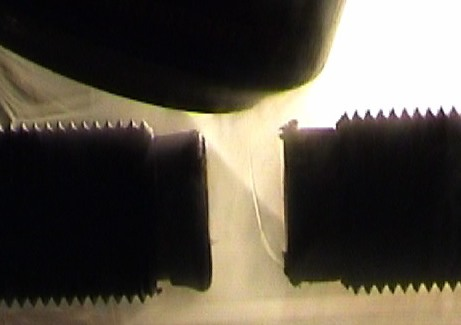
\includegraphics[width=0.42\linewidth]{images/book3/liquid-oxygen.jpg}

{\small Un fino chorro de oxígeno líquido que cae entre los polos de un imán potente
es atraído hacia ellos y queda suspendido como un puente: la molécula es
\omterm{def:b2:diatomic-mos:magnetism}{paramagnética}. (Fotografía: Pieter Kuiper, dominio público, Wikimedia Commons.)}
\end{omfigure}

\section{El método CLOA}

\begin{definition}[Orbital molecular]\label{def:b2:diatomic-mos:lcao}
Un \emph{orbital molecular}\index{orbital molecular} es la \omterm{def:b2:atomic-orbitals:wavefunction}{función de onda} de un
electrón en una molécula, extendida sobre todos sus núcleos. En el método \emph{CLOA}\index{CLOA}
(combinación lineal de orbitales atómicos) se escribe como una suma de orbitales atómicos
de los átomos, $\psi = \sum_i c_i\varphi_i$, con coeficientes elegidos para
que la energía sea mínima.
\end{definition}

Para dos átomos A y B que aportan cada uno un orbital, $\psi = c_A\varphi_A + c_B\varphi_B$.
La energía de un electrón en $\psi$, minimizada respecto de los coeficientes,
hace intervenir tres números.

\begin{definition}[Las integrales del método CLOA]\label{def:b2:diatomic-mos:integrals}
Para dos orbitales atómicos reales $\varphi_A$, $\varphi_B$ y el operador energía $\hat H$
de un electrón en la molécula:
\begin{itemize}
  \item la \emph{integral de solapamiento}\index{integral de solapamiento} $S = \int\varphi_A\varphi_B\,dV$
        mide en qué medida los dos orbitales ocupan la misma región ($S = 1$ para
        orbitales idénticos y superpuestos);
  \item la \emph{integral de Coulomb}\index{integral de Coulomb} $\alpha_A = \int\varphi_A\hat
        H\varphi_A\,dV$ es la energía de un electrón en $\varphi_A$ dentro de la molécula,
        próxima a la energía del orbital atómico;
  \item la \emph{integral de resonancia}\index{integral de resonancia} $\beta = \int\varphi_A\hat
        H\varphi_B\,dV$, negativa, mide el acoplamiento de los dos orbitales.
\end{itemize}
Las energías $E$ de los \omterm{def:b2:diatomic-mos:lcao}{orbitales moleculares} son las raíces del \emph{determinante
secular}\index{determinante secular}
\[
  \begin{vmatrix} \alpha_A - E & \beta - ES \\ \beta - ES & \alpha_B - E \end{vmatrix} = 0 .
\]
\end{definition}

El determinante procede de minimizar $E = \int\psi\hat H\psi\,dV/\int\psi^2\,dV$
respecto de $c_A$ y $c_B$: las dos condiciones $\partial E/\partial c_A =
\partial E/\partial c_B = 0$ forman un sistema lineal homogéneo, que solo tiene una solución
no nula cuando su determinante se anula. Ese paso variacional se admite
aquí.

\begin{theorem}[Dos orbitales idénticos]\label{thm:b2:diatomic-mos:homonuclear}
Para $\alpha_A = \alpha_B = \alpha$, los dos \omterm{def:b2:diatomic-mos:lcao}{orbitales moleculares} son
\[
  E_+ = \frac{\alpha + \beta}{1 + S}, \quad \psi_+ = \frac{\varphi_A + \varphi_B}{\sqrt{2(1 + S)}} ;
  \qquad
  E_- = \frac{\alpha - \beta}{1 - S}, \quad \psi_- = \frac{\varphi_A - \varphi_B}{\sqrt{2(1 - S)}} .
\]
\end{theorem}

\begin{proof}
El determinante da $(\alpha - E)^2 = (\beta - ES)^2$, luego $\alpha - E = \pm(\beta - ES)$.
Con el signo más, $E(1 + S) = \alpha + \beta$; con el signo menos, $E(1 - S) = \alpha
- \beta$. Volviendo al sistema lineal, $(\alpha - E)c_A + (\beta - ES)c_B = 0$ da $c_B
= c_A$ para $E_+$ y $c_B = -c_A$ para $E_-$. Normalización: $\int(\varphi_A \pm
\varphi_B)^2\,dV = 2 \pm 2S$.
\end{proof}

\begin{definition}[Orbitales enlazantes y antienlazantes]\label{def:b2:diatomic-mos:bonding}
Un \emph{orbital enlazante}\index{orbital enlazante} está por debajo de los orbitales atómicos
que lo forman: su densidad electrónica se acumula entre los núcleos. Un
\emph{orbital antienlazante}\index{orbital antienlazante} está por encima de ellos y tiene un
plano nodal entre los núcleos. Un \emph{orbital no enlazante}\index{orbital no enlazante}
conserva la energía del orbital atómico, que no encuentra pareja con la que
combinarse.
\end{definition}

\begin{proposition}[El orbital antienlazante sube más]\label{prop:b2:diatomic-mos:asymmetry}
Para $S > 0$, el nivel antienlazante sube por encima de $\alpha$ más de lo que
baja el nivel enlazante por debajo.
\end{proposition}

\begin{proof}
$E_+ - \alpha = (\beta - \alpha S)/(1 + S)$ y $E_- - \alpha = -(\beta - \alpha S)/(1 - S)$.
El numerador $\beta - \alpha S$ es negativo (domina el acoplamiento), y $1 - S < 1
+ S$: el segundo desplazamiento es mayor en valor absoluto.
\end{proof}

Con dos electrones, como en \ce{H2}, ambos entran en $\psi_+$ y la molécula es más
estable que los átomos separados. Con cuatro, como en \ce{He2}, dos deben entrar en $\psi_-$,
lo que cuesta más de lo que gana $\psi_+$: \ce{He2} no está ligado.

\begin{omfigure}
\begin{MOdiagram}[names, labels]
  \atom[H]{left}{ 1s = {0;up} }
  \atom[H]{right}{ 1s = {0;up} }
  \molecule[\ce{H2}]{ 1sMO = {.75;pair} }
\end{MOdiagram}
\hspace{1.5cm}
\begin{MOdiagram}[names, labels]
  \atom[He]{left}{ 1s = {0;pair} }
  \atom[He]{right}{ 1s = {0;pair} }
  \molecule[\ce{He2}]{ 1sMO = {.75;pair,pair} }
\end{MOdiagram}

{\small Diagramas de \omterm{def:b2:diatomic-mos:lcao}{orbitales moleculares} de \ce{H2} (\omterm{def:b2:diatomic-mos:bond-order}{orden de enlace} 1) y de \ce{He2} (\omterm{def:b2:diatomic-mos:bond-order}{orden
de enlace} 0, no ligado). Cada casilla es un nivel que contiene como mucho dos electrones de
espines opuestos; las líneas discontinuas unen cada \omterm{def:b2:diatomic-mos:lcao}{orbital molecular} con los orbitales atómicos
a partir de los que se construye.}
\end{omfigure}

\section{Solapamiento y simetría}

\begin{definition}[Orbitales $\sigma$ y $\pi$]\label{def:b2:diatomic-mos:sigma-pi}
Un \emph{orbital $\sigma$}\index{orbital sigma@orbital $\sigma$} de una molécula lineal no cambia con ninguna
rotación alrededor del eje molecular: no tiene ningún plano nodal que contenga el eje. Un
\emph{orbital $\pi$}\index{orbital pi@orbital $\pi$} cambia de signo con una rotación de $180^\circ$ alrededor del
eje: tiene un plano nodal que contiene el eje. Un asterisco señala los \omterm{def:b2:diatomic-mos:bonding}{orbitales
antienlazantes} ($\sigma^*$, $\pi^*$).
\end{definition}

\begin{proposition}[Solapamiento nulo por simetría]\label{prop:b2:diatomic-mos:symmetry}
Dos orbitales de los que uno es simétrico y el otro antisimétrico respecto
de un plano que contiene el eje molecular tienen solapamiento nulo e \omterm{def:b2:diatomic-mos:integrals}{integral de resonancia}
nula: no se combinan.
\end{proposition}

\begin{proof}
La reflexión en el plano deja el espacio invariante pero convierte el producto
$\varphi_A\varphi_B$ en su opuesto en el punto simétrico: las contribuciones de las
dos mitades del espacio a $\int\varphi_A\varphi_B\,dV$ se cancelan. Lo mismo vale para
$\int\varphi_A\hat H\varphi_B\,dV$, ya que $\hat H$ tiene la simetría de la molécula.
\end{proof}

Dos orbitales interaccionan fuertemente cuando tienen la misma simetría (solapamiento
no nulo), se solapan bien y están a energías próximas. Un orbital 1s de un átomo y un
$2\mathrm p_x$ del otro ($x$ perpendicular al eje) nunca se combinan;
los orbitales $2\mathrm p_z$ (a lo largo del eje) dan orbitales $\sigma$; los $2\mathrm p_x$ y
$2\mathrm p_y$ dan dos pares de orbitales $\pi$ de igual energía.

\begin{omfigure}
\begin{tikzpicture}[font=\small]
  % sigma 1s
  \pic at (0,0) {oms={0.85}}; \pic at (0.7,0) {oms={0.85}};
  \node at (0.35,-0.75) {$\sigma_{1s}$};
  \pic at (2.2,0) {oms={0.85}}; \pic at (2.9,0) {oms={-0.85}};
  \node at (2.55,-0.75) {$\sigma^*_{1s}$};
  % sigma 2p
  \pic at (4.6,0) {omp={-1}{0}}; \pic at (5.6,0) {omp={1}{0}};
  \node at (5.1,-0.75) {$\sigma_{2p}$};
  \pic at (7.4,0) {omp={-1}{0}}; \pic at (8.6,0) {omp={-1}{0}};
  \node at (8.0,-0.75) {$\sigma^*_{2p}$};
  % pi 2p
  \pic at (10.2,0) {omp={1}{90}}; \pic at (10.9,0) {omp={1}{90}};
  \node at (10.55,-0.95) {$\pi_{2p}$};
  \pic at (12.2,0) {omp={1}{90}}; \pic at (12.9,0) {omp={-1}{90}};
  \node at (12.55,-0.95) {$\pi^*_{2p}$};
  \draw[black!40, dashed] (-0.6,0) -- (13.4,0);
\end{tikzpicture}

{\small \omterm{def:b2:diatomic-mos:lcao}{Orbitales moleculares} de una molécula diatómica homonuclear, esquema (el eje
molecular es horizontal y discontinuo). Las combinaciones en fase (enlazantes) reúnen el
mismo color entre los núcleos; las combinaciones en oposición de fase (antienlazantes) ponen un
plano nodal entre ellos. Los orbitales $\sigma$ son simétricos respecto del eje; cada orbital $\pi$
tiene el eje en su plano nodal.}
\end{omfigure}

\section{Moléculas diatómicas homonucleares del periodo 2}

Con los orbitales 2s y 2p de dos átomos del periodo 2 se forman ocho \omterm{def:b2:diatomic-mos:lcao}{orbitales moleculares}:
$\sigma_{2s}$, $\sigma^*_{2s}$, $\sigma_{2p}$, dos $\pi_{2p}$, dos $\pi^*_{2p}$ y
$\sigma^*_{2p}$.

\begin{proposition}[Mezcla s--p]\label{prop:b2:diatomic-mos:sp-mixing}
Para \ce{O2} y \ce{F2} el orden es $\sigma_{2s} < \sigma^*_{2s} < \sigma_{2p} < \pi_{2p} <
\pi^*_{2p} < \sigma^*_{2p}$. Para \ce{Li2} a \ce{N2}, cuyos niveles 2s y 2p están próximos,
los orbitales $\sigma$ formados a partir de 2s y $2\mathrm p_z$ se mezclan: $\sigma_{2p}$ sube por encima de
$\pi_{2p}$.
\end{proposition}

\begin{proof}[Argumento]
Los orbitales $\sigma_{2s}$ y $\sigma_{2p}$ tienen la misma simetría y pueden combinarse
entre sí. Dos niveles de la misma simetría se repelen (\cref{thm:b2:diatomic-mos:heteronuclear},
más abajo): $\sigma_{2s}$ baja y $\sigma_{2p}$ sube, tanto más cuanto más próximos están. La
diferencia 2s--2p crece a lo largo del periodo, de modo que el efecto es grande a la izquierda y pequeño para
el oxígeno y el flúor. El cruce entre el nitrógeno y el oxígeno se admite a partir de los
espectros fotoelectrónicos medidos.
\end{proof}

\begin{definition}[Orden de enlace]\label{def:b2:diatomic-mos:bond-order}
El \emph{orden de enlace}\index{orden de enlace} de una molécula diatómica es $b = (n_b -
n_a)/2$, donde $n_b$ y $n_a$ son los números de electrones en \omterm{def:b2:diatomic-mos:bonding}{orbitales enlazantes} y
antienlazantes.
\end{definition}

\begin{proposition}[Orden de enlace y enlace]\label{prop:b2:diatomic-mos:bond-order}
Entre átomos del mismo par de elementos, un \omterm{def:b2:diatomic-mos:bond-order}{orden de enlace} mayor va acompañado de un
enlace más corto y más fuerte; un \omterm{def:b2:diatomic-mos:bond-order}{orden de enlace} nulo significa que no hay enlace.
\end{proposition}

\begin{proof}[Argumento]
Cada electrón enlazante añade densidad entre los núcleos y rebaja la energía;
cada electrón antienlazante la retira y eleva la energía al menos otro tanto
(\cref{prop:b2:diatomic-mos:asymmetry}). El número neto de pares enlazantes mide
la unión. La comparación solo tiene sentido para átomos parecidos: \ce{Li2} tiene
\omterm{def:b2:diatomic-mos:bond-order}{orden de enlace} 1, como \ce{F2}, pero sus orbitales 2s son mucho mayores.
\end{proof}

\begin{definition}[Paramagnético y diamagnético]\label{def:b2:diatomic-mos:magnetism}
Una sustancia es \emph{paramagnética}\index{paramagnetica@paramagnética} si sus moléculas tienen
electrones desapareados: es atraída hacia un campo magnético. Es
\emph{diamagnética}\index{diamagnetica@diamagnética} si todos sus electrones están apareados: es
débilmente repelida por el campo.
\end{definition}

\begin{omfigure}
\begin{MOdiagram}[names, labels, style=square, distance=4.2cm, labels-fs=\scriptsize]
  \atom[N]{left}{ 2s = {0;pair}, 2p = {3.5;up,up,up} }
  \atom[N]{right}{ 2s = {0;pair}, 2p = {3.5;up,up,up} }
  \molecule[\ce{N2}]{ 2sMO = {.7;pair,pair}, 2pMO = {0.4/2.5,1.4;pair,pair,pair} }
\end{MOdiagram}
\hfill
\begin{MOdiagram}[names, labels, style=square, distance=4.2cm, labels-fs=\scriptsize]
  \atom[O]{left}{ 2s = {0;pair}, 2p = {3.5;pair,up,up} }
  \atom[O]{right}{ 2s = {0;pair}, 2p = {3.5;pair,up,up} }
  \molecule[\ce{O2}]{ 2sMO = {.7;pair,pair}, 2pMO = {1.8,.8;pair,pair,pair,up,up} }
\end{MOdiagram}

{\small Diagramas de \omterm{def:b2:diatomic-mos:lcao}{orbitales moleculares} de valencia de \ce{N2} (a la izquierda, con mezcla s--p:
$\sigma_{2p}$ por encima de $\pi_{2p}$) y de \ce{O2} (a la derecha). Nitrógeno: \omterm{def:b2:diatomic-mos:bond-order}{orden de enlace}
$(8 - 2)/2 = 3$, todos los electrones apareados. Oxígeno: \omterm{def:b2:diatomic-mos:bond-order}{orden de enlace} $(8 - 4)/2 = 2$, con dos
electrones desapareados en los dos orbitales $\pi^*$ (regla de Hund): \ce{O2} es
\omterm{def:b2:diatomic-mos:magnetism}{paramagnético}. Los diagramas toman $x$ como eje molecular; de ahí las etiquetas
$2\sigma_x$, $2\pi_y$, $2\pi_z$.}
\end{omfigure}

\begin{method}[Construir y llenar un diagrama de OM]\label{met:b2:diatomic-mos:build-diagram}
\begin{enumerate}
  \item Sitúense los orbitales atómicos de valencia de cada átomo a su energía, el átomo
        más electronegativo más abajo.
  \item Combínense los orbitales de la misma simetría: cada par da un \omterm{def:b2:diatomic-mos:bonding}{orbital enlazante}
        por debajo y un \omterm{def:b2:diatomic-mos:bonding}{orbital antienlazante} por encima; un orbital sin pareja queda
        no enlazante.
  \item Para las moléculas homonucleares del periodo 2, úsese el orden con $\sigma_{2p}$ por encima de
        $\pi_{2p}$ hasta el nitrógeno, y por debajo a partir del oxígeno.
\end{enumerate}
\end{method}

\begin{method}[Leer un diagrama lleno]\label{met:b2:diatomic-mos:fill}
\begin{enumerate}
  \item Cuéntense los electrones de valencia (súmese uno por cada carga negativa y réstese uno
        por cada carga positiva).
  \item Llénese desde abajo, dos por orbital, con la regla de Hund para los niveles
        degenerados.
  \item \omterm{def:b2:diatomic-mos:bond-order}{Orden de enlace} $(n_b - n_a)/2$; los electrones desapareados dan paramagnetismo.
  \item El nivel ocupado más alto es el que se ioniza primero.
\end{enumerate}
\end{method}

\begin{omfigure}
\small
\renewcommand{\arraystretch}{1.15}
\begin{tabular}{lcccccc}
 & \ce{Li2} & \ce{C2} & \ce{N2} & \ce{O2} & \ce{F2} & \ce{NO} \\ \hline
electrones de valencia & 2 & 8 & 10 & 12 & 14 & 11 \\
\omterm{def:b2:diatomic-mos:bond-order}{orden de enlace} & 1 & 2 & 3 & 2 & 1 & 2.5 \\
electrones desapareados & 0 & 0 & 0 & 2 & 0 & 1 \\
longitud de enlace $r_e$ (pm) & 267.3 & 124.3 & 109.8 & 120.8 & 141.2 & 115.1 \\
$D_0$ (\unit{eV}) & 1.04 & 6.15 & 9.76 & 5.12 & 1.60 & 6.51 \\
\end{tabular}

\smallskip
{\small Moléculas diatómicas del periodo 2: \omterm{def:b2:diatomic-mos:bond-order}{órdenes de enlace} según los diagramas de OM; longitudes de enlace
espectroscópicas, y energías de disociación $D_0$ a partir de entalpías de formación tabuladas
a \qty{0}{K}, $D_0 = \Delta_f H_0(\mathrm A) + \Delta_f H_0(\mathrm B) - \Delta_f
H_0(\mathrm{AB})$.}
% ledger: re:Li2, re:C2, re:N2, re:O2, re:F2, re:NO, janafH0:Li, janafH0:Li2, janafH0:C, janafH0:C2, janafH0:N, janafH0:O, janafH0:F, janafH0:NO
\end{omfigure}

\section{Moléculas diatómicas heteronucleares}

\begin{theorem}[Dos orbitales de energías distintas]\label{thm:b2:diatomic-mos:heteronuclear}
Para $\alpha_A > \alpha_B$ (B más electronegativo), despreciando $S$, con $\bar\alpha = (\alpha_A
+ \alpha_B)/2$ y $\Delta = \alpha_A - \alpha_B$:
\[
  E_\mp = \bar\alpha \mp \sqrt{\Delta^2/4 + \beta^2} .
\]
El \omterm{def:b2:diatomic-mos:bonding}{orbital enlazante} (más bajo) tiene su coeficiente mayor sobre B, y el \omterm{def:b2:diatomic-mos:bonding}{orbital
antienlazante}, sobre A; cuando $\Delta \gg |\beta|$, $E_- \approx \alpha_B - \beta^2/\Delta$ y $E_+
\approx \alpha_A + \beta^2/\Delta$.
\end{theorem}

\begin{proof}
Con $S = 0$ las energías son los valores propios de $\begin{pmatrix}\alpha_A & \beta \\
\beta & \alpha_B\end{pmatrix}$: $(\alpha_A - E)(\alpha_B - E) = \beta^2$, cuyas raíces son
$\bar\alpha \pm \sqrt{\Delta^2/4 + \beta^2}$. Para la raíz menor, $(\alpha_B - E_-)c_B = -\beta
c_A$; $\alpha_B - E_- = \sqrt{\Delta^2/4 + \beta^2} - \Delta/2$ es menor que $|\beta|$, luego
$|c_A| < |c_B|$. Para $\Delta \gg |\beta|$, $\sqrt{\Delta^2/4 + \beta^2} \approx \Delta/2 +
\beta^2/\Delta$.
\end{proof}

\begin{omfigure}
\begin{tikzpicture}
\begin{axis}[width=0.55\linewidth, height=6cm, xmin=0, xmax=8, ymin=-5, ymax=5,
  axis x line=bottom, axis y line=left, xlabel={$\Delta/|\beta|$}, ylabel={$E/|\beta|$},
  tick label style={font=\small}, label style={font=\small}]
\addplot[omThm, thick] table[x=d, y=Ehigh] {figdata/out/bachelor-2-two-level-a.dat};
\addplot[omDef, thick] table[x=d, y=Elow] {figdata/out/bachelor-2-two-level-a.dat};
\addplot[black!50, densely dotted] table[x=d, y=aA] {figdata/out/bachelor-2-two-level-a.dat};
\addplot[black!50, densely dotted] table[x=d, y=aB] {figdata/out/bachelor-2-two-level-a.dat};
\addplot[omThm, dashed] table[x=d, y=Phigh] {figdata/out/bachelor-2-two-level-a-pert.dat};
\addplot[omDef, dashed] table[x=d, y=Plow] {figdata/out/bachelor-2-two-level-a-pert.dat};
\node[font=\scriptsize, black!60, anchor=north west] at (axis cs:5.5,2.6) {$\alpha_A$};
\node[font=\scriptsize, black!60, anchor=south west] at (axis cs:5.5,-2.6) {$\alpha_B$};
\node[font=\scriptsize, omThm, anchor=south east] at (axis cs:3.2,2.2) {antienlazante};
\node[font=\scriptsize, omDef, anchor=north east] at (axis cs:3.2,-2.2) {enlazante};
\end{axis}
\end{tikzpicture}

{\small Dos niveles que interaccionan. A medida que crece la diferencia $\Delta$ entre los orbitales atómicos,
los niveles moleculares (trazo continuo) se acercan a los atómicos (punteados): la estabilización
$\beta^2/\Delta$ del límite perturbativo (discontinuo) se vuelve pequeña. Para $\Delta = 0$ el
desdoblamiento es $2|\beta|$.}
\end{omfigure}

En el fluoruro de hidrógeno, el orbital 1s del hidrógeno se encuentra con los orbitales 2p, mucho más bajos,
del flúor. Solo el $2\mathrm p_z$, a lo largo del eje, tiene la simetría adecuada: forma
un \omterm{def:b2:diatomic-mos:bonding}{orbital enlazante} $\sigma$ con más peso sobre el flúor, y un $\sigma^*$ con más peso sobre el
hidrógeno. Los orbitales $2\mathrm p_x$ y $2\mathrm p_y$ del flúor permanecen
no enlazantes: son sus pares no enlazantes. El enlace está polarizado hacia el flúor.

El monóxido de carbono tiene los diez electrones de valencia de \ce{N2} y un diagrama parecido,
pero los orbitales del oxígeno están más bajos. Sus \omterm{def:b2:diatomic-mos:bonding}{orbitales enlazantes} tienen más peso sobre el oxígeno;
su orbital ocupado más alto, un orbital $\sigma$ con más peso sobre el carbono, es un par no enlazante
del carbono. Por eso el monóxido de carbono se une a los metales por el carbono
(\cref{ch:b2:coordination-complexes}).

\begin{omfigure}
\begin{tikzpicture}[font=\small]
  % CO schematic: C left (higher), O right (lower)
  \pic (c2s) at (0,0.6) {omlevel={ud}{0.8}}; \node[left] at (-0.5,0.6) {2s};
  \pic (c2p1) at (-0.45,2.6) {omlevel={u}{0.4}}; \pic (c2p2) at (0,2.6) {omlevel={u}{0.4}}; \pic (c2p3) at (0.45,2.6) {omlevel={empty}{0.4}};
  \node[left] at (-0.75,2.6) {2p};
  \node at (0,-0.6) {C};
  \pic (o2s) at (6,-1.2) {omlevel={ud}{0.8}}; \node[right] at (6.5,-1.2) {2s};
  \pic (o2p1) at (5.55,1.4) {omlevel={ud}{0.4}}; \pic (o2p2) at (6,1.4) {omlevel={u}{0.4}}; \pic (o2p3) at (6.45,1.4) {omlevel={u}{0.4}};
  \node[right] at (6.75,1.4) {2p};
  \node at (6,-2.2) {O};
  % MOs
  \pic (m1) at (3,-1.8) {omlevel={ud}{0.8}};
  \pic (m2) at (3,-0.2) {omlevel={ud}{0.8}};
  \pic (m3a) at (2.75,0.9) {omlevel={ud}{0.45}}; \pic (m3b) at (3.25,0.9) {omlevel={ud}{0.45}};
  \pic (m4) at (3,1.9) {omlevel={ud}{0.8}};
  \pic (m5a) at (2.75,3.3) {omlevel={empty}{0.45}}; \pic (m5b) at (3.25,3.3) {omlevel={empty}{0.45}};
  \pic (m6) at (3,4.4) {omlevel={empty}{0.8}};
  \draw[omcorr, densely dashed] (c2s-r) -- (m1-l) (o2s-l) -- (m1-r);
  \draw[omcorr, densely dashed] (c2s-r) -- (m2-l) (o2s-l) -- (m2-r);
  \draw[omcorr, densely dashed] (c2p3-r) -- (m3a-l) (o2p1-l) -- (m3b-r);
  \draw[omcorr, densely dashed] (c2p3-r) -- (m4-l) (o2p1-l) -- (m4-r);
  \draw[omcorr, densely dashed] (c2p3-r) -- (m5a-l) (o2p1-l) -- (m5b-r);
  \draw[omcorr, densely dashed] (c2p3-r) -- (m6-l) (o2p1-l) -- (m6-r);
  \node[omsymlabel, below=0.17cm, inner sep=0.5pt] at (m1-c) {$\sigma$};
  \node[omsymlabel, below=0.17cm, inner sep=0.5pt] at (m2-c) {$\sigma$};
  \node[omsymlabel, below=0.17cm, inner sep=0.5pt] at (3,0.9) {$\pi$};
  \node[omsymlabel, below=0.24cm, inner sep=0.5pt] at (m4-c) {$\sigma$ (par libre de C)};
  \node[omsymlabel, below=0.05cm, inner sep=0.5pt] at (3,3.3) {$\pi^*$};
  \node[omsymlabel, below=0.05cm, inner sep=0.5pt] at (m6-c) {$\sigma^*$};
  \node at (3,-2.6) {CO};
\end{tikzpicture}

{\small Orbitales de valencia del monóxido de carbono, esquema: los orbitales del oxígeno están
más bajos que los del carbono. \omterm{def:b2:diatomic-mos:bond-order}{Orden de enlace} 3, como en \ce{N2}; el orbital ocupado
más alto es un orbital $\sigma$ con más peso sobre el carbono, su par no enlazante.}
\end{omfigure}

\begin{history}[Hund y Mulliken]
\begin{minipage}[t]{0.27\linewidth}
\vspace{0pt}
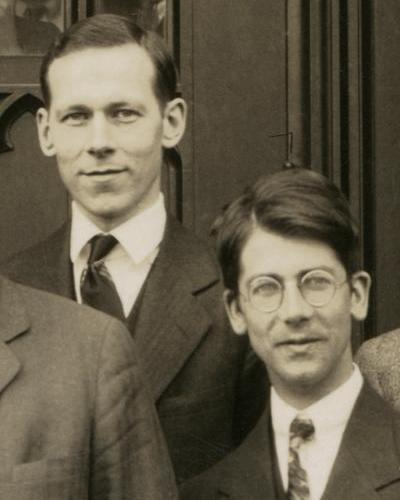
\includegraphics[width=\linewidth]{images/book3/mulliken-hund.jpg}
\end{minipage}\hfill
\begin{minipage}[t]{0.69\linewidth}
\vspace{0pt}
Entre 1926 y 1932, Friedrich Hund y Robert Mulliken interpretaron los espectros
de las moléculas diatómicas asignando cada electrón a un orbital de toda la
molécula, clasificado según su simetría respecto del eje. Los términos $\sigma$, $\pi$,
enlazante y antienlazante, y los diagramas de orbitales de este capítulo proceden de su
trabajo; Mulliken recibió el Premio Nobel de Química en 1966. La fotografía muestra a
Mulliken (a la izquierda) y a Hund en Chicago en 1929. (Fotografía: GFHund, CC BY 3.0,
Wikimedia Commons.)
\end{minipage}
\end{history}

\section{Ionización y fuerza del enlace}

Arrancar un electrón de un \omterm{def:b2:diatomic-mos:bonding}{orbital enlazante} debilita el enlace; arrancarlo de
un \omterm{def:b2:diatomic-mos:bonding}{orbital antienlazante} lo refuerza. Las energías de disociación de los iones
se obtienen de un ciclo termoquímico: para $\mathrm{AB}^+ \to \mathrm A + \mathrm B^+$,
\[
  D_0(\mathrm{AB}^+) = D_0(\mathrm{AB}) + I(\mathrm B) - I(\mathrm{AB}) ,
\]
siendo B el átomo de menor energía de ionización.

\begin{example}[Iones del nitrógeno y del oxígeno]\label{ex:b2:diatomic-mos:ions}
\ce{N2} ($I = \qty{15.58}{eV}$) pierde un electrón enlazante: $D_0(\ce{N2+}) = 9.76 + 14.53 -
15.58 = \qty{8.71}{eV}$, más débil que \ce{N2}. \ce{O2} ($I = \qty{12.07}{eV}$) pierde un
electrón $\pi^*$: $D_0(\ce{O2+}) = 5.12 + 13.62 - 12.07 = \qty{6.66}{eV}$, más fuerte que \ce{O2},
de acuerdo con los \omterm{def:b2:diatomic-mos:bond-order}{órdenes de enlace} 2.5 y 2.5 frente a 3 y 2.
% ledger: ie:N2, ie:N, ie:O2, ie:O, janafH0:N, janafH0:O
\end{example}

\section{Ejercicios}

\begin{exercise}[$\star$]\label{exo:b2:diatomic-mos:1}
Para dos orbitales 1s del hidrógeno tómense $\alpha = \qty{-13.6}{eV}$, $\beta = \qty{-9.0}{eV}$ y
$S = 0.60$ (datos del ejercicio). Calcúlense $E_+$ y $E_-$, y después la energía de los dos
electrones de \ce{H2} comparada con la de dos átomos separados.
\end{exercise}

\begin{exercise}[$\star$]\label{exo:b2:diatomic-mos:2}
Dense los \omterm{def:b2:diatomic-mos:bond-order}{órdenes de enlace} de \ce{He2}, \ce{He2+}, \ce{Li2} y \ce{B2} (con mezcla
s--p).
\end{exercise}

\begin{exercise}[$\star$]\label{exo:b2:diatomic-mos:3}
¿Cuáles de \ce{B2}, \ce{C2}, \ce{N2}, \ce{O2}, \ce{F2} son \omterm{def:b2:diatomic-mos:magnetism}{paramagnéticas}?
\end{exercise}

\begin{exercise}[$\star$]\label{exo:b2:diatomic-mos:4}
El eje molecular es $z$. ¿Qué pares entre (1s, $2\mathrm p_z$), (1s,
$2\mathrm p_x$), ($2\mathrm p_x$, $2\mathrm p_x$), ($2\mathrm p_x$, $2\mathrm p_y$),
(2s, $2\mathrm p_z$) tienen solapamiento no nulo?
\end{exercise}

\begin{exercise}[$\star\star$]\label{exo:b2:diatomic-mos:5}
Prevéase si \ce{N2+} tiene un enlace más largo o más corto que \ce{N2}, y compruébese con
su energía de disociación calculada en el capítulo.
\end{exercise}

\begin{exercise}[$\star\star$]\label{exo:b2:diatomic-mos:6}
El monóxido de carbono y \ce{N2} son isoelectrónicos. Explíquese por qué los \omterm{def:b2:diatomic-mos:bonding}{orbitales enlazantes} del
CO tienen más peso sobre el oxígeno y por qué su orbital ocupado más alto es un par no enlazante del
carbono.
\end{exercise}

\begin{exercise}[$\star\star$]\label{exo:b2:diatomic-mos:7}
En el HF, ¿qué orbitales del flúor interaccionan con el 1s del hidrógeno y cuáles permanecen
no enlazantes? Dibújese el diagrama.
\end{exercise}

\begin{exercise}[$\star\star$]\label{exo:b2:diatomic-mos:8}
Con $\alpha_A = \qty{-10}{eV}$, $\alpha_B = \qty{-14}{eV}$ y $\beta = \qty{-3.0}{eV}$
(datos del ejercicio, $S$ despreciada), calcúlense las dos energías y el peso $c_B^2$ del
\omterm{def:b2:diatomic-mos:bonding}{orbital enlazante} sobre B.
\end{exercise}

\begin{exercise}[$\star\star$]\label{exo:b2:diatomic-mos:9}
Con mezcla s--p, demuéstrese que \ce{C2} tiene un \omterm{def:b2:diatomic-mos:bond-order}{orden de enlace} 2 formado por dos enlaces $\pi$ y ningún
enlace $\sigma_{2p}$.
\end{exercise}

\begin{exercise}[$\star\star\star$]\label{exo:b2:diatomic-mos:10}
Dense los \omterm{def:b2:diatomic-mos:bond-order}{órdenes de enlace} de NO y de \ce{NO+}. A partir de $D_0(\ce{NO}) = \qty{6.51}{eV}$, $I(\ce{NO}) =
\qty{9.26}{eV}$ e $I(\ce{O}) = \qty{13.62}{eV}$, calcúlese $D_0(\ce{NO+})$ para $\ce{NO+} \to
\ce{N} + \ce{O+}$, y coméntese.
\end{exercise}

\begin{exercise}[$\star\star\star$]\label{exo:b2:diatomic-mos:11}
Demuéstrese que $E_+ + E_- = 2(\alpha - \beta S)/(1 - S^2)$, y que supera $2\alpha$ cuando
$\beta < \alpha S < 0$. Dedúzcase por qué dos orbitales llenos se repelen (desestabilización a cuatro
electrones).
\end{exercise}

\begin{exercise}[$\star\star\star$]\label{exo:b2:diatomic-mos:12}
Ordénense \ce{O2+}, \ce{O2}, \ce{O2-}, \ce{O2^2-} por \omterm{def:b2:diatomic-mos:bond-order}{orden de enlace}, longitud de enlace y fuerza
del enlace. ¿Qué ion se encuentra en el peróxido de hidrógeno, y cuál en el compuesto
amarillo \ce{KO2}?
\end{exercise}

\section{Problema: el oxígeno y sus iones}

\begin{problem}[{Problema de fin de semana --- el diagrama de orbitales moleculares del dioxígeno,
los órdenes de enlace y el magnetismo de sus iones, la ionización y la fuerza del
enlace, y las dos maneras de aparear los electrones $\pi^*$}]
\label{pb:b2:diatomic-mos:1}
Datos: $I(\ce{O}) = \qty{13.62}{eV}$, $I(\ce{O2}) = \qty{12.07}{eV}$, $I(\ce{N}) =
\qty{14.53}{eV}$, $I(\ce{N2}) = \qty{15.58}{eV}$; $\Delta_f H_0$ a \qty{0}{K}
(\unit{kJ/mol}): \ce{O} 246.79, \ce{N} 470.82; $r_e$: \ce{O2} \qty{120.8}{pm}, \ce{N2}
\qty{109.8}{pm}; $1\ \unit{eV} = \qty{96.485}{kJ/mol}$.
% ledger: ie:O, ie:O2, ie:N, ie:N2, janafH0:O, janafH0:N, re:O2, re:N2

\medskip
\noindent\textbf{Parte I --- El dioxígeno.}
\begin{enumerate}
  \item ¿Cuántos electrones de valencia tiene \ce{O2}?
  \item Dibújese su diagrama de OM de valencia (sin mezcla s--p) y llénese.
  \item Calcúlese su \omterm{def:b2:diatomic-mos:bond-order}{orden de enlace}.
  \item ¿Cuántos electrones desapareados tiene? ¿Es \ce{O2} \omterm{def:b2:diatomic-mos:magnetism}{paramagnético}?
  \item ¿Por qué falla aquí la estructura de Lewis?
  \item Calcúlese $D_0(\ce{O2})$ en \unit{eV}.
\end{enumerate}

\medskip
\noindent\textbf{Parte II --- Los iones.}
\begin{enumerate}[resume]
  \item Dense la configuración y el \omterm{def:b2:diatomic-mos:bond-order}{orden de enlace} de \ce{O2+}.
  \item Lo mismo para el ion superóxido \ce{O2-}.
  \item Lo mismo para el ion peróxido \ce{O2^2-}.
  \item Dese el número de electrones desapareados de cada ion.
  \item Ordénense \ce{O2+}, \ce{O2}, \ce{O2-}, \ce{O2^2-} según la longitud de enlace prevista.
  \item ¿Qué ion tiene un enlace sencillo O--O, como el peróxido de hidrógeno?
  \item ¿Cuáles de las cuatro especies son \omterm{def:b2:diatomic-mos:magnetism}{paramagnéticas}?
\end{enumerate}

\medskip
\noindent\textbf{Parte III --- Ionización.}
\begin{enumerate}[resume]
  \item ¿De qué orbital sale el electrón cuando se ioniza \ce{O2}?
  \item ¿Por qué es $I(\ce{O2})$ menor que $I(\ce{O})$?
  \item Demuéstrese que $D_0(\ce{O2+}) = D_0(\ce{O2}) + I(\ce{O}) - I(\ce{O2})$ y calcúlese.
  \item Compárese con $D_0(\ce{O2})$ y explíquese.
  \item Calcúlense del mismo modo $D_0(\ce{N2})$ y $D_0(\ce{N2+})$.
  \item ¿Por qué es $I(\ce{N2})$ mayor que $I(\ce{N})$?
  \item Resúmase: ¿cuándo refuerza la ionización un enlace?
\end{enumerate}

\medskip
\noindent\textbf{Parte IV --- Los electrones $\pi^*$.}
\begin{enumerate}[resume]
  \item En el estado fundamental los dos electrones $\pi^*$ ocupan dos orbitales distintos con
        espines paralelos. ¿Qué regla lo dice?
  \item Descríbase un estado en el que ambos ocupan el mismo orbital $\pi^*$.
  \item ¿Por qué ese estado tiene más energía?
  \item ¿Cuáles son su \omterm{def:b2:diatomic-mos:bond-order}{orden de enlace} y su magnetismo?
  \item Indíquense el \omterm{def:b2:diatomic-mos:bond-order}{orden de enlace} de \ce{O2+} y su energía de disociación.
\end{enumerate}
\end{problem}
